\documentclass[1p]{elsarticle_modified}
%\bibliographystyle{elsarticle-num}

%\usepackage[colorlinks]{hyperref}
%\usepackage{abbrmath_seonhwa} %\Abb, \Ascr, \Acal ,\Abf, \Afrak
\usepackage{amsfonts}
\usepackage{amssymb}
\usepackage{amsmath}
\usepackage{amsthm}
\usepackage{scalefnt}
\usepackage{amsbsy}
\usepackage{kotex}
\usepackage{caption}
\usepackage{subfig}
\usepackage{color}
\usepackage{graphicx}
\usepackage{xcolor} %% white, black, red, green, blue, cyan, magenta, yellow
\usepackage{float}
\usepackage{setspace}
\usepackage{hyperref}

\usepackage{tikz}
\usetikzlibrary{arrows}

\usepackage{multirow}
\usepackage{array} % fixed length table
\usepackage{hhline}

%%%%%%%%%%%%%%%%%%%%%
\makeatletter
\renewcommand*\env@matrix[1][\arraystretch]{%
	\edef\arraystretch{#1}%
	\hskip -\arraycolsep
	\let\@ifnextchar\new@ifnextchar
	\array{*\c@MaxMatrixCols c}}
\makeatother %https://tex.stackexchange.com/questions/14071/how-can-i-increase-the-line-spacing-in-a-matrix
%%%%%%%%%%%%%%%

\usepackage[normalem]{ulem}

\newcommand{\msout}[1]{\ifmmode\text{\sout{\ensuremath{#1}}}\else\sout{#1}\fi}
%SOURCE: \msout is \stkout macro in https://tex.stackexchange.com/questions/20609/strikeout-in-math-mode

\newcommand{\cancel}[1]{
	\ifmmode
	{\color{red}\msout{#1}}
	\else
	{\color{red}\sout{#1}}
	\fi
}

\newcommand{\add}[1]{
	{\color{blue}\uwave{#1}}
}

\newcommand{\replace}[2]{
	\ifmmode
	{\color{red}\msout{#1}}{\color{blue}\uwave{#2}}
	\else
	{\color{red}\sout{#1}}{\color{blue}\uwave{#2}}
	\fi
}

\newcommand{\Sol}{\mathcal{S}} %segment
\newcommand{\D}{D} %diagram
\newcommand{\A}{\mathcal{A}} %arc


%%%%%%%%%%%%%%%%%%%%%%%%%%%%%5 test

\def\sl{\operatorname{\textup{SL}}(2,\Cbb)}
\def\psl{\operatorname{\textup{PSL}}(2,\Cbb)}
\def\quan{\mkern 1mu \triangleright \mkern 1mu}

\theoremstyle{definition}
\newtheorem{thm}{Theorem}[section]
\newtheorem{prop}[thm]{Proposition}
\newtheorem{lem}[thm]{Lemma}
\newtheorem{ques}[thm]{Question}
\newtheorem{cor}[thm]{Corollary}
\newtheorem{defn}[thm]{Definition}
\newtheorem{exam}[thm]{Example}
\newtheorem{rmk}[thm]{Remark}
\newtheorem{alg}[thm]{Algorithm}

\newcommand{\I}{\sqrt{-1}}
\begin{document}

%\begin{frontmatter}
%
%\title{Boundary parabolic representations of knots up to 8 crossings}
%
%%% Group authors per affiliation:
%\author{Yunhi Cho} 
%\address{Department of Mathematics, University of Seoul, Seoul, Korea}
%\ead{yhcho@uos.ac.kr}
%
%
%\author{Seonhwa Kim} %\fnref{s_kim}}
%\address{Center for Geometry and Physics, Institute for Basic Science, Pohang, 37673, Korea}
%\ead{ryeona17@ibs.re.kr}
%
%\author{Hyuk Kim}
%\address{Department of Mathematical Sciences, Seoul National University, Seoul 08826, Korea}
%\ead{hyukkim@snu.ac.kr}
%
%\author{Seokbeom Yoon}
%\address{Department of Mathematical Sciences, Seoul National University, Seoul, 08826,  Korea}
%\ead{sbyoon15@snu.ac.kr}
%
%\begin{abstract}
%We find all boundary parabolic representation of knots up to 8 crossings.
%
%\end{abstract}
%\begin{keyword}
%    \MSC[2010] 57M25 
%\end{keyword}
%
%\end{frontmatter}

%\linenumbers
%\tableofcontents
%
\newcommand\colored[1]{\textcolor{white}{\rule[-0.35ex]{0.8em}{1.4ex}}\kern-0.8em\color{red} #1}%
%\newcommand\colored[1]{\textcolor{white}{ #1}\kern-2.17ex	\textcolor{white}{ #1}\kern-1.81ex	\textcolor{white}{ #1}\kern-2.15ex\color{red}#1	}

{\Large $\underline{12a_{1183}~(K12a_{1183})}$}

\setlength{\tabcolsep}{10pt}
\renewcommand{\arraystretch}{1.6}
\vspace{1cm}\begin{tabular}{m{100pt}>{\centering\arraybackslash}m{274pt}}
\multirow{5}{120pt}{
	\centering
	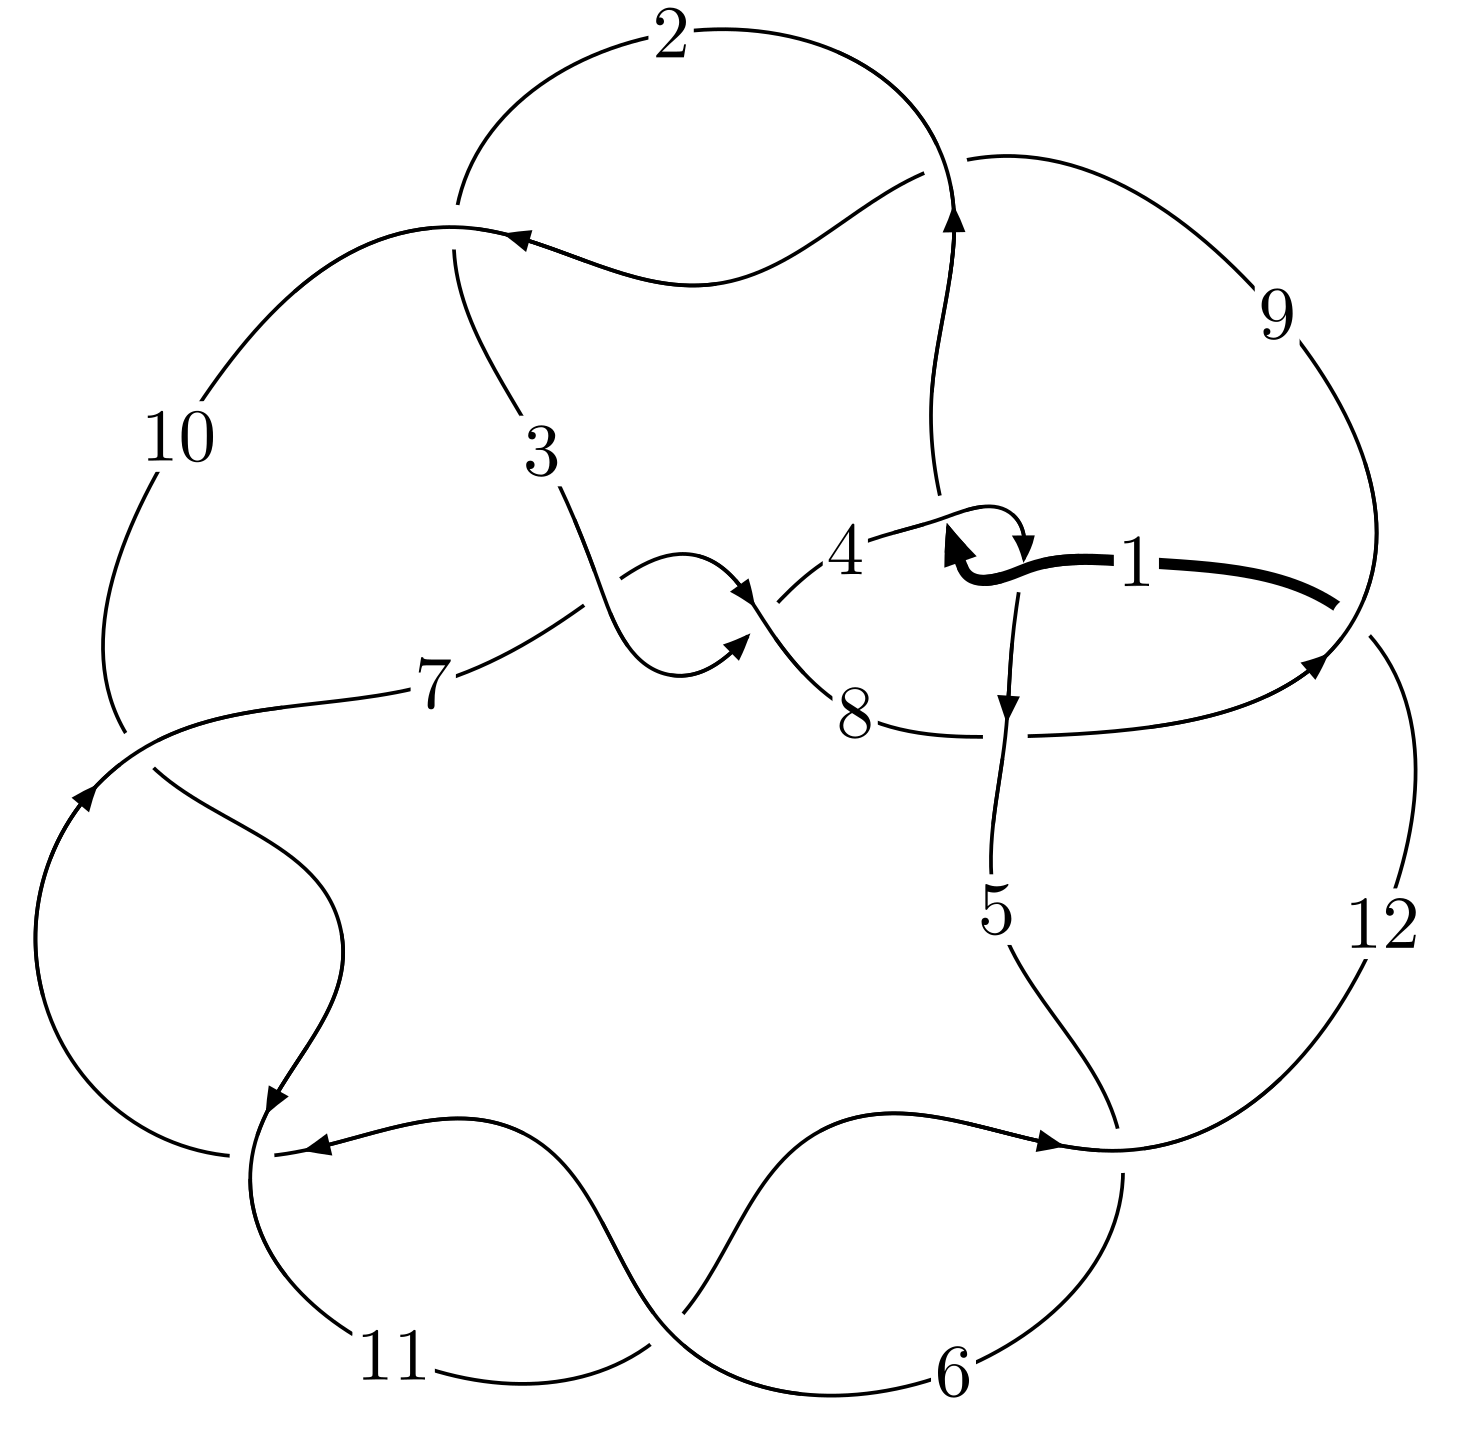
\includegraphics[width=112pt]{../../../GIT/diagram.site/Diagrams/png/1984_12a_1183.png}\\
\ \ \ A knot diagram\footnotemark}&
\allowdisplaybreaks
\textbf{Linearized knot diagam} \\
\cline{2-2}
 &
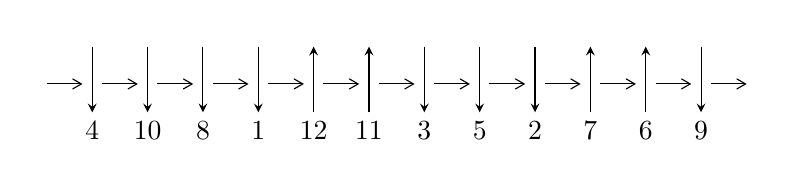
\begin{tikzpicture}[x=20pt, y=17pt]
	% nodes
	\node (C0) at (0, 0) {};
	\node (C1) at (1, 0) {};
	\node (C1U) at (1, +1) {};
	\node (C1D) at (1, -1) {4};

	\node (C2) at (2, 0) {};
	\node (C2U) at (2, +1) {};
	\node (C2D) at (2, -1) {10};

	\node (C3) at (3, 0) {};
	\node (C3U) at (3, +1) {};
	\node (C3D) at (3, -1) {8};

	\node (C4) at (4, 0) {};
	\node (C4U) at (4, +1) {};
	\node (C4D) at (4, -1) {1};

	\node (C5) at (5, 0) {};
	\node (C5U) at (5, +1) {};
	\node (C5D) at (5, -1) {12};

	\node (C6) at (6, 0) {};
	\node (C6U) at (6, +1) {};
	\node (C6D) at (6, -1) {11};

	\node (C7) at (7, 0) {};
	\node (C7U) at (7, +1) {};
	\node (C7D) at (7, -1) {3};

	\node (C8) at (8, 0) {};
	\node (C8U) at (8, +1) {};
	\node (C8D) at (8, -1) {5};

	\node (C9) at (9, 0) {};
	\node (C9U) at (9, +1) {};
	\node (C9D) at (9, -1) {2};

	\node (C10) at (10, 0) {};
	\node (C10U) at (10, +1) {};
	\node (C10D) at (10, -1) {7};

	\node (C11) at (11, 0) {};
	\node (C11U) at (11, +1) {};
	\node (C11D) at (11, -1) {6};

	\node (C12) at (12, 0) {};
	\node (C12U) at (12, +1) {};
	\node (C12D) at (12, -1) {9};
	\node (C13) at (13, 0) {};

	% arrows
	\draw[->,>={angle 60}]
	(C0) edge (C1) (C1) edge (C2) (C2) edge (C3) (C3) edge (C4) (C4) edge (C5) (C5) edge (C6) (C6) edge (C7) (C7) edge (C8) (C8) edge (C9) (C9) edge (C10) (C10) edge (C11) (C11) edge (C12) (C12) edge (C13) ;	\draw[->,>=stealth]
	(C1U) edge (C1D) (C2U) edge (C2D) (C3U) edge (C3D) (C4U) edge (C4D) (C5D) edge (C5U) (C6D) edge (C6U) (C7U) edge (C7D) (C8U) edge (C8D) (C9U) edge (C9D) (C10D) edge (C10U) (C11D) edge (C11U) (C12U) edge (C12D) ;
	\end{tikzpicture} \\
\hhline{~~} \\& 
\textbf{Solving Sequence} \\ \cline{2-2} 
 &
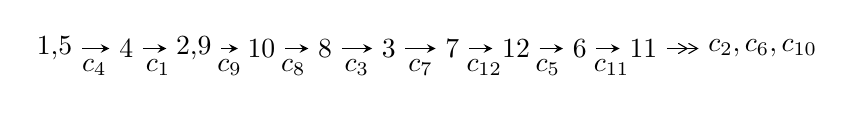
\begin{tikzpicture}[x=23pt, y=7pt]
	% node
	\node (A0) at (-1/8, 0) {1,5};
	\node (A1) at (1, 0) {4};
	\node (A2) at (33/16, 0) {2,9};
	\node (A3) at (25/8, 0) {10};
	\node (A4) at (33/8, 0) {8};
	\node (A5) at (41/8, 0) {3};
	\node (A6) at (49/8, 0) {7};
	\node (A7) at (57/8, 0) {12};
	\node (A8) at (65/8, 0) {6};
	\node (A9) at (73/8, 0) {11};
	\node (C1) at (1/2, -1) {$c_{4}$};
	\node (C2) at (3/2, -1) {$c_{1}$};
	\node (C3) at (21/8, -1) {$c_{9}$};
	\node (C4) at (29/8, -1) {$c_{8}$};
	\node (C5) at (37/8, -1) {$c_{3}$};
	\node (C6) at (45/8, -1) {$c_{7}$};
	\node (C7) at (53/8, -1) {$c_{12}$};
	\node (C8) at (61/8, -1) {$c_{5}$};
	\node (C9) at (69/8, -1) {$c_{11}$};
	\node (A10) at (11, 0) {$c_{2},c_{6},c_{10}$};

	% edge
	\draw[->,>=stealth]	
	(A0) edge (A1) (A1) edge (A2) (A2) edge (A3) (A3) edge (A4) (A4) edge (A5) (A5) edge (A6) (A6) edge (A7) (A7) edge (A8) (A8) edge (A9) ;
	\draw[->>,>={angle 60}]	
	(A9) edge (A10);
\end{tikzpicture} \\ 

\end{tabular} \\

\footnotetext{
The image of knot diagram is generated by the software ``\textbf{Draw programme}" developed by Andrew Bartholomew(\url{http://www.layer8.co.uk/maths/draw/index.htm\#Running-draw}), where we modified some parts for our purpose(\url{https://github.com/CATsTAILs/LinksPainter}).
}\phantom \\ \newline 
\centering \textbf{Ideals for irreducible components\footnotemark of $X_{\text{par}}$} 
 
\begin{align*}
I^u_{1}&=\langle 
7 u^{26}-128 u^{25}+\cdots+8 b+328,\;-41 u^{26}+628 u^{25}+\cdots+32 a+816,\;u^{27}-16 u^{26}+\cdots+448 u-32\rangle \\
I^u_{2}&=\langle 
3830888122431 a^9 u^4-2857501004595 a^8 u^4+\cdots+8963993636290 a-1366272633452,\\
\phantom{I^u_{2}}&\phantom{= \langle  }- a^9 u^4-4 a^8 u^4+\cdots-5 a-10,\;u^5+u^4+2 u^3+u^2+u+1\rangle \\
I^u_{3}&=\langle 
4 u^{16}+12 u^{15}+\cdots+b-2,\;2 u^{16}+18 u^{15}+\cdots+3 a+32,\;u^{17}+3 u^{16}+\cdots+7 u+3\rangle \\
\\
\end{align*}
\raggedright * 3 irreducible components of $\dim_{\mathbb{C}}=0$, with total 94 representations.\\
\footnotetext{All coefficients of polynomials are rational numbers. But the coefficients are sometimes approximated in decimal forms when there is not enough margin.}
\newpage
\renewcommand{\arraystretch}{1}
\centering \section*{I. $I^u_{1}= \langle 7 u^{26}-128 u^{25}+\cdots+8 b+328,\;-41 u^{26}+628 u^{25}+\cdots+32 a+816,\;u^{27}-16 u^{26}+\cdots+448 u-32 \rangle$}
\flushleft \textbf{(i) Arc colorings}\\
\begin{tabular}{m{7pt} m{180pt} m{7pt} m{180pt} }
\flushright $a_{1}=$&$\begin{pmatrix}0\\u\end{pmatrix}$ \\
\flushright $a_{5}=$&$\begin{pmatrix}1\\0\end{pmatrix}$ \\
\flushright $a_{4}=$&$\begin{pmatrix}1\\- u^2\end{pmatrix}$ \\
\flushright $a_{2}=$&$\begin{pmatrix}- u\\u^3+u\end{pmatrix}$ \\
\flushright $a_{9}=$&$\begin{pmatrix}1.28125 u^{26}-19.6250 u^{25}+\cdots+254.500 u-25.5000\\-\frac{7}{8} u^{26}+16 u^{25}+\cdots+\frac{1199}{2} u-41\end{pmatrix}$ \\
\flushright $a_{10}=$&$\begin{pmatrix}-1.46875 u^{26}+22.1250 u^{25}+\cdots+361.500 u-29.5000\\-\frac{9}{8} u^{26}+\frac{57}{4} u^{25}+\cdots-\frac{855}{2} u+35\end{pmatrix}$ \\
\flushright $a_{8}=$&$\begin{pmatrix}\frac{13}{32} u^{26}-\frac{29}{8} u^{25}+\cdots+854 u-\frac{133}{2}\\-\frac{7}{8} u^{26}+16 u^{25}+\cdots+\frac{1199}{2} u-41\end{pmatrix}$ \\
\flushright $a_{3}=$&$\begin{pmatrix}\frac{1}{32} u^{26}-\frac{5}{16} u^{25}+\cdots+33 u-2\\-\frac{9}{16} u^{26}+\frac{69}{8} u^{25}+\cdots+250 u-19\end{pmatrix}$ \\
\flushright $a_{7}=$&$\begin{pmatrix}-2.68750 u^{26}+44.4375 u^{25}+\cdots+1475.75 u-109.500\\-\frac{61}{16} u^{26}+\frac{449}{8} u^{25}+\cdots+\frac{777}{2} u-24\end{pmatrix}$ \\
\flushright $a_{12}=$&$\begin{pmatrix}\frac{45}{32} u^{26}-\frac{337}{16} u^{25}+\cdots-233 u+15\\-\frac{23}{16} u^{26}+\frac{179}{8} u^{25}+\cdots+616 u-45\end{pmatrix}$ \\
\flushright $a_{6}=$&$\begin{pmatrix}\frac{53}{32} u^{26}-\frac{213}{8} u^{25}+\cdots-\frac{821}{2} u+25\\\frac{3}{4} u^{26}-\frac{81}{8} u^{25}+\cdots+119 u-7\end{pmatrix}$ \\
\flushright $a_{11}=$&$\begin{pmatrix}-\frac{11}{4} u^{26}+\frac{309}{8} u^{25}+\cdots-967 u+82\\\frac{33}{8} u^{26}-\frac{519}{8} u^{25}+\cdots-1569 u+110\end{pmatrix}$\\&\end{tabular}
\flushleft \textbf{(ii) Obstruction class $= -1$}\\~\\
\flushleft \textbf{(iii) Cusp Shapes $= -\frac{9}{4} u^{26}+37 u^{25}+\cdots+348 u-10$}\\~\\
\newpage\renewcommand{\arraystretch}{1}
\flushleft \textbf{(iv) u-Polynomials at the component}\newline \\
\begin{tabular}{m{50pt}|m{274pt}}
Crossings & \hspace{64pt}u-Polynomials at each crossing \\
\hline $$\begin{aligned}c_{1},c_{4}\end{aligned}$$&$\begin{aligned}
&u^{27}-16 u^{26}+\cdots+448 u-32
\end{aligned}$\\
\hline $$\begin{aligned}c_{2},c_{3},c_{7}\\c_{9}\end{aligned}$$&$\begin{aligned}
&u^{27}- u^{26}+\cdots+4 u^2+1
\end{aligned}$\\
\hline $$\begin{aligned}c_{5},c_{6},c_{10}\\c_{11}\end{aligned}$$&$\begin{aligned}
&u^{27}-11 u^{26}+\cdots+416 u-32
\end{aligned}$\\
\hline $$\begin{aligned}c_{8},c_{12}\end{aligned}$$&$\begin{aligned}
&u^{27}+u^{26}+\cdots+5 u+1
\end{aligned}$\\
\hline
\end{tabular}\\~\\
\newpage\renewcommand{\arraystretch}{1}
\flushleft \textbf{(v) Riley Polynomials at the component}\newline \\
\begin{tabular}{m{50pt}|m{274pt}}
Crossings & \hspace{64pt}Riley Polynomials at each crossing \\
\hline $$\begin{aligned}c_{1},c_{4}\end{aligned}$$&$\begin{aligned}
&y^{27}+16 y^{26}+\cdots-9728 y-1024
\end{aligned}$\\
\hline $$\begin{aligned}c_{2},c_{3},c_{7}\\c_{9}\end{aligned}$$&$\begin{aligned}
&y^{27}-27 y^{26}+\cdots-8 y-1
\end{aligned}$\\
\hline $$\begin{aligned}c_{5},c_{6},c_{10}\\c_{11}\end{aligned}$$&$\begin{aligned}
&y^{27}+31 y^{26}+\cdots-3584 y-1024
\end{aligned}$\\
\hline $$\begin{aligned}c_{8},c_{12}\end{aligned}$$&$\begin{aligned}
&y^{27}-5 y^{26}+\cdots+3 y-1
\end{aligned}$\\
\hline
\end{tabular}\\~\\
\newpage\flushleft \textbf{(vi) Complex Volumes and Cusp Shapes}
$$\begin{array}{c|c|c}  
\text{Solutions to }I^u_{1}& \I (\text{vol} + \sqrt{-1}CS) & \text{Cusp shape}\\
 \hline 
\begin{aligned}
u &= \phantom{-}0.326738 + 0.973251 I \\
a &= \phantom{-}1.36638 - 0.75273 I \\
b &= -1.17904 - 1.08389 I\end{aligned}
 & -5.90216 - 5.12959 I & -5.71356 - 0.71345 I \\ \hline\begin{aligned}
u &= \phantom{-}0.326738 - 0.973251 I \\
a &= \phantom{-}1.36638 + 0.75273 I \\
b &= -1.17904 + 1.08389 I\end{aligned}
 & -5.90216 + 5.12959 I & -5.71356 + 0.71345 I \\ \hline\begin{aligned}
u &= \phantom{-}0.257668 + 1.013350 I \\
a &= -1.094370 + 0.580330 I \\
b &= \phantom{-}0.870061 + 0.959444 I\end{aligned}
 & \phantom{-}1.67867 - 3.20907 I & -3.00867 + 3.20014 I \\ \hline\begin{aligned}
u &= \phantom{-}0.257668 - 1.013350 I \\
a &= -1.094370 - 0.580330 I \\
b &= \phantom{-}0.870061 - 0.959444 I\end{aligned}
 & \phantom{-}1.67867 + 3.20907 I & -3.00867 - 3.20014 I \\ \hline\begin{aligned}
u &= \phantom{-}0.156189 + 1.077390 I \\
a &= \phantom{-}0.815391 - 0.397247 I \\
b &= -0.555344 - 0.816446 I\end{aligned}
 & \phantom{-}3.09390 + 0.00363 I & \phantom{-}1.18580 - 2.67864 I \\ \hline\begin{aligned}
u &= \phantom{-}0.156189 - 1.077390 I \\
a &= \phantom{-}0.815391 + 0.397247 I \\
b &= -0.555344 + 0.816446 I\end{aligned}
 & \phantom{-}3.09390 - 0.00363 I & \phantom{-}1.18580 + 2.67864 I \\ \hline\begin{aligned}
u &= \phantom{-}1.165660 + 0.184416 I \\
a &= -0.911038 + 0.705453 I \\
b &= \phantom{-}1.192060 - 0.654307 I\end{aligned}
 & -19.4453 + 9.1728 I & -13.26883 - 4.48783 I \\ \hline\begin{aligned}
u &= \phantom{-}1.165660 - 0.184416 I \\
a &= -0.911038 - 0.705453 I \\
b &= \phantom{-}1.192060 + 0.654307 I\end{aligned}
 & -19.4453 - 9.1728 I & -13.26883 + 4.48783 I \\ \hline\begin{aligned}
u &= -0.135256 + 1.225450 I \\
a &= -0.369172 + 0.209810 I \\
b &= \phantom{-}0.207180 + 0.480781 I\end{aligned}
 & -0.53153 + 2.11620 I & -4.00000 - 3.37376 I \\ \hline\begin{aligned}
u &= -0.135256 - 1.225450 I \\
a &= -0.369172 - 0.209810 I \\
b &= \phantom{-}0.207180 - 0.480781 I\end{aligned}
 & -0.53153 - 2.11620 I & -4.00000 + 3.37376 I\\
 \hline 
 \end{array}$$\newpage$$\begin{array}{c|c|c}  
\text{Solutions to }I^u_{1}& \I (\text{vol} + \sqrt{-1}CS) & \text{Cusp shape}\\
 \hline 
\begin{aligned}
u &= \phantom{-}1.296730 + 0.234088 I \\
a &= \phantom{-}0.629855 - 0.468322 I \\
b &= -0.926383 + 0.459847 I\end{aligned}
 & -9.64040 + 5.83308 I & -13.1962 - 6.2251 I \\ \hline\begin{aligned}
u &= \phantom{-}1.296730 - 0.234088 I \\
a &= \phantom{-}0.629855 + 0.468322 I \\
b &= -0.926383 - 0.459847 I\end{aligned}
 & -9.64040 - 5.83308 I & -13.1962 + 6.2251 I \\ \hline\begin{aligned}
u &= \phantom{-}0.401898 + 0.513270 I \\
a &= \phantom{-}0.05616 - 1.60013 I \\
b &= -0.843872 + 0.614264 I\end{aligned}
 & -7.16168 + 2.04670 I & -4.62828 - 4.92551 I \\ \hline\begin{aligned}
u &= \phantom{-}0.401898 - 0.513270 I \\
a &= \phantom{-}0.05616 + 1.60013 I \\
b &= -0.843872 - 0.614264 I\end{aligned}
 & -7.16168 - 2.04670 I & -4.62828 + 4.92551 I \\ \hline\begin{aligned}
u &= \phantom{-}0.63266 + 1.30092 I \\
a &= -1.110240 + 0.483598 I \\
b &= \phantom{-}1.33153 + 1.13838 I\end{aligned}
 & -15.9655 - 15.4642 I & \phantom{-0.000000 } 0 \\ \hline\begin{aligned}
u &= \phantom{-}0.63266 - 1.30092 I \\
a &= -1.110240 - 0.483598 I \\
b &= \phantom{-}1.33153 - 1.13838 I\end{aligned}
 & -15.9655 + 15.4642 I & \phantom{-0.000000 } 0 \\ \hline\begin{aligned}
u &= \phantom{-}0.67380 + 1.29759 I \\
a &= \phantom{-}0.990312 - 0.341657 I \\
b &= -1.11060 - 1.05481 I\end{aligned}
 & -6.30603 - 12.55790 I & \phantom{-0.000000 } 0 \\ \hline\begin{aligned}
u &= \phantom{-}0.67380 - 1.29759 I \\
a &= \phantom{-}0.990312 + 0.341657 I \\
b &= -1.11060 + 1.05481 I\end{aligned}
 & -6.30603 + 12.55790 I & \phantom{-0.000000 } 0 \\ \hline\begin{aligned}
u &= \phantom{-}0.75681 + 1.30765 I \\
a &= -0.790458 + 0.172262 I \\
b &= \phantom{-}0.823487 + 0.903270 I\end{aligned}
 & -2.55975 - 7.75483 I & \phantom{-0.000000 } 0 \\ \hline\begin{aligned}
u &= \phantom{-}0.75681 - 1.30765 I \\
a &= -0.790458 - 0.172262 I \\
b &= \phantom{-}0.823487 - 0.903270 I\end{aligned}
 & -2.55975 + 7.75483 I & \phantom{-0.000000 } 0\\
 \hline 
 \end{array}$$\newpage$$\begin{array}{c|c|c}  
\text{Solutions to }I^u_{1}& \I (\text{vol} + \sqrt{-1}CS) & \text{Cusp shape}\\
 \hline 
\begin{aligned}
u &= \phantom{-}1.58357\phantom{ +0.000000I} \\
a &= -0.438551\phantom{ +0.000000I} \\
b &= \phantom{-}0.694476\phantom{ +0.000000I}\end{aligned}
 & -6.13943\phantom{ +0.000000I} & \phantom{-0.000000 } 0 \\ \hline\begin{aligned}
u &= \phantom{-}0.202392 + 0.231714 I \\
a &= \phantom{-}0.26309 + 1.63520 I \\
b &= \phantom{-}0.325651 - 0.391913 I\end{aligned}
 & -0.150445 + 0.974739 I & -2.92263 - 7.14002 I \\ \hline\begin{aligned}
u &= \phantom{-}0.202392 - 0.231714 I \\
a &= \phantom{-}0.26309 - 1.63520 I \\
b &= \phantom{-}0.325651 + 0.391913 I\end{aligned}
 & -0.150445 - 0.974739 I & -2.92263 + 7.14002 I \\ \hline\begin{aligned}
u &= \phantom{-}0.89228 + 1.45430 I \\
a &= \phantom{-}0.440805 - 0.117681 I \\
b &= -0.564466 - 0.536060 I\end{aligned}
 & -4.37833 - 2.08868 I & \phantom{-0.000000 } 0 \\ \hline\begin{aligned}
u &= \phantom{-}0.89228 - 1.45430 I \\
a &= \phantom{-}0.440805 + 0.117681 I \\
b &= -0.564466 + 0.536060 I\end{aligned}
 & -4.37833 + 2.08868 I & \phantom{-0.000000 } 0 \\ \hline\begin{aligned}
u &= \phantom{-}0.58063 + 1.74046 I \\
a &= -0.067440 + 0.312189 I \\
b &= \phantom{-}0.582509 - 0.063892 I\end{aligned}
 & -13.55330 + 2.79514 I & \phantom{-0.000000 } 0 \\ \hline\begin{aligned}
u &= \phantom{-}0.58063 - 1.74046 I \\
a &= -0.067440 - 0.312189 I \\
b &= \phantom{-}0.582509 + 0.063892 I\end{aligned}
 & -13.55330 - 2.79514 I & \phantom{-0.000000 } 0\\
 \hline 
 \end{array}$$\newpage\newpage\renewcommand{\arraystretch}{1}
\centering \section*{II. $I^u_{2}= \langle 3.83\times10^{12} a^{9} u^{4}-2.86\times10^{12} a^{8} u^{4}+\cdots+8.96\times10^{12} a-1.37\times10^{12},\;- a^9 u^4-4 a^8 u^4+\cdots-5 a-10,\;u^5+u^4+2 u^3+u^2+u+1 \rangle$}
\flushleft \textbf{(i) Arc colorings}\\
\begin{tabular}{m{7pt} m{180pt} m{7pt} m{180pt} }
\flushright $a_{1}=$&$\begin{pmatrix}0\\u\end{pmatrix}$ \\
\flushright $a_{5}=$&$\begin{pmatrix}1\\0\end{pmatrix}$ \\
\flushright $a_{4}=$&$\begin{pmatrix}1\\- u^2\end{pmatrix}$ \\
\flushright $a_{2}=$&$\begin{pmatrix}- u\\u^3+u\end{pmatrix}$ \\
\flushright $a_{9}=$&$\begin{pmatrix}a\\-1.30396 a^{9} u^{4}+0.972636 a^{8} u^{4}+\cdots-3.05116 a+0.465052\end{pmatrix}$ \\
\flushright $a_{10}=$&$\begin{pmatrix}-1.34977 a^{9} u^{4}+2.51833 a^{8} u^{4}+\cdots+0.382620 a+0.196848\\0.275845 a^{9} u^{4}+1.98098 a^{8} u^{4}+\cdots-0.891259 a+0.748114\end{pmatrix}$ \\
\flushright $a_{8}=$&$\begin{pmatrix}-1.30396 a^{9} u^{4}+0.972636 a^{8} u^{4}+\cdots-2.05116 a+0.465052\\-1.30396 a^{9} u^{4}+0.972636 a^{8} u^{4}+\cdots-3.05116 a+0.465052\end{pmatrix}$ \\
\flushright $a_{3}=$&$\begin{pmatrix}0.978965 a^{9} u^{4}-1.44213 a^{8} u^{4}+\cdots-0.0881825 a+0.194750\\-0.311779 a^{9} u^{4}-0.827493 a^{8} u^{4}+\cdots-0.104852 a-0.728899\end{pmatrix}$ \\
\flushright $a_{7}=$&$\begin{pmatrix}-1.32778 a^{9} u^{4}+0.504526 a^{8} u^{4}+\cdots-0.111225 a-0.415918\\-3.49328 a^{9} u^{4}+0.486696 a^{8} u^{4}+\cdots+1.37737 a-1.28533\end{pmatrix}$ \\
\flushright $a_{12}=$&$\begin{pmatrix}a^2 u\\1.16482 a^{9} u^{4}-0.841308 a^{8} u^{4}+\cdots-0.639242 a+0.155880\end{pmatrix}$ \\
\flushright $a_{6}=$&$\begin{pmatrix}0.598958 a^{9} u^{4}-0.536641 a^{8} u^{4}+\cdots-0.100841 a+0.898935\\2.00856 a^{9} u^{4}-0.391347 a^{8} u^{4}+\cdots-0.420272 a+1.38748\end{pmatrix}$ \\
\flushright $a_{11}=$&$\begin{pmatrix}-0.269881 a^{9} u^{4}-0.151648 a^{8} u^{4}+\cdots+0.391092 a-0.370194\\-2.37370 a^{9} u^{4}+2.91763 a^{8} u^{4}+\cdots+0.705077 a-0.305615\end{pmatrix}$\\&\end{tabular}
\flushleft \textbf{(ii) Obstruction class $= -1$}\\~\\
\flushleft \textbf{(iii) Cusp Shapes $= -\frac{3336817308298}{1468946744399} a^9 u^4+\frac{8995916260558}{1468946744399} a^8 u^4+\cdots-\frac{6523463258754}{1468946744399} a-\frac{5778728076718}{1468946744399}$}\\~\\
\newpage\renewcommand{\arraystretch}{1}
\flushleft \textbf{(iv) u-Polynomials at the component}\newline \\
\begin{tabular}{m{50pt}|m{274pt}}
Crossings & \hspace{64pt}u-Polynomials at each crossing \\
\hline $$\begin{aligned}c_{1},c_{4}\end{aligned}$$&$\begin{aligned}
&(u^5+u^4+2 u^3+u^2+u+1)^{10}
\end{aligned}$\\
\hline $$\begin{aligned}c_{2},c_{3},c_{7}\\c_{9}\end{aligned}$$&$\begin{aligned}
&u^{50}- u^{49}+\cdots+3504 u-928
\end{aligned}$\\
\hline $$\begin{aligned}c_{5},c_{6},c_{10}\\c_{11}\end{aligned}$$&$\begin{aligned}
&(u^5+u^4+4 u^3+3 u^2+3 u+1)^{10}
\end{aligned}$\\
\hline $$\begin{aligned}c_{8},c_{12}\end{aligned}$$&$\begin{aligned}
&u^{50}+5 u^{49}+\cdots-80 u-32
\end{aligned}$\\
\hline
\end{tabular}\\~\\
\newpage\renewcommand{\arraystretch}{1}
\flushleft \textbf{(v) Riley Polynomials at the component}\newline \\
\begin{tabular}{m{50pt}|m{274pt}}
Crossings & \hspace{64pt}Riley Polynomials at each crossing \\
\hline $$\begin{aligned}c_{1},c_{4}\end{aligned}$$&$\begin{aligned}
&(y^5+3 y^4+4 y^3+y^2- y-1)^{10}
\end{aligned}$\\
\hline $$\begin{aligned}c_{2},c_{3},c_{7}\\c_{9}\end{aligned}$$&$\begin{aligned}
&y^{50}-45 y^{49}+\cdots-84632320 y+861184
\end{aligned}$\\
\hline $$\begin{aligned}c_{5},c_{6},c_{10}\\c_{11}\end{aligned}$$&$\begin{aligned}
&(y^5+7 y^4+16 y^3+13 y^2+3 y-1)^{10}
\end{aligned}$\\
\hline $$\begin{aligned}c_{8},c_{12}\end{aligned}$$&$\begin{aligned}
&y^{50}-9 y^{49}+\cdots-40704 y+1024
\end{aligned}$\\
\hline
\end{tabular}\\~\\
\newpage\flushleft \textbf{(vi) Complex Volumes and Cusp Shapes}
$$\begin{array}{c|c|c}  
\text{Solutions to }I^u_{2}& \I (\text{vol} + \sqrt{-1}CS) & \text{Cusp shape}\\
 \hline 
\begin{aligned}
u &= \phantom{-}0.339110 + 0.822375 I \\
a &= -0.941072 - 0.102065 I \\
b &= \phantom{-}1.188350 - 0.588608 I\end{aligned}
 & -3.72352 - 1.53058 I & -3.87605 + 4.43065 I \\ \hline\begin{aligned}
u &= \phantom{-}0.339110 + 0.822375 I \\
a &= \phantom{-}0.368837 - 1.146040 I \\
b &= -0.40610 - 1.63231 I\end{aligned}
 & -6.42551 + 0.68339 I & -12.37057 + 0.20776 I \\ \hline\begin{aligned}
u &= \phantom{-}0.339110 + 0.822375 I \\
a &= -0.630435 + 1.098070 I \\
b &= \phantom{-}0.63922 + 2.16713 I\end{aligned}
 & -15.5640 + 1.8012 I & -13.40362 + 2.06837 I \\ \hline\begin{aligned}
u &= \phantom{-}0.339110 + 0.822375 I \\
a &= \phantom{-}0.10246 + 1.48727 I \\
b &= \phantom{-}0.235191 + 0.808525 I\end{aligned}
 & -3.72352 - 1.53058 I & -3.87605 + 4.43065 I \\ \hline\begin{aligned}
u &= \phantom{-}0.339110 + 0.822375 I \\
a &= \phantom{-}0.051054 + 0.421661 I \\
b &= \phantom{-}2.04277 - 1.49049 I\end{aligned}
 & -15.5640 - 4.8623 I & -13.4036 + 6.7929 I \\ \hline\begin{aligned}
u &= \phantom{-}0.339110 + 0.822375 I \\
a &= \phantom{-}0.255094 - 0.199412 I \\
b &= -1.62129 + 1.17233 I\end{aligned}
 & -6.42551 - 3.74455 I & -12.3706 + 8.6535 I \\ \hline\begin{aligned}
u &= \phantom{-}0.339110 + 0.822375 I \\
a &= \phantom{-}1.87045 + 0.27748 I \\
b &= -1.067550 + 0.085312 I\end{aligned}
 & -6.42551 + 0.68339 I & -12.37057 + 0.20776 I \\ \hline\begin{aligned}
u &= \phantom{-}0.339110 + 0.822375 I \\
a &= -0.52357 - 2.18737 I \\
b &= -0.250496 - 0.142160 I\end{aligned}
 & -6.42551 - 3.74455 I & -12.3706 + 8.6535 I \\ \hline\begin{aligned}
u &= \phantom{-}0.339110 + 0.822375 I \\
a &= -2.52618 - 0.26440 I \\
b &= \phantom{-}1.116810 + 0.146089 I\end{aligned}
 & -15.5640 + 1.8012 I & -13.40362 + 2.06837 I \\ \hline\begin{aligned}
u &= \phantom{-}0.339110 + 0.822375 I \\
a &= \phantom{-}0.67360 + 2.76175 I \\
b &= \phantom{-}0.329451 - 0.184975 I\end{aligned}
 & -15.5640 - 4.8623 I & -13.4036 + 6.7929 I\\
 \hline 
 \end{array}$$\newpage$$\begin{array}{c|c|c}  
\text{Solutions to }I^u_{2}& \I (\text{vol} + \sqrt{-1}CS) & \text{Cusp shape}\\
 \hline 
\begin{aligned}
u &= \phantom{-}0.339110 - 0.822375 I \\
a &= -0.941072 + 0.102065 I \\
b &= \phantom{-}1.188350 + 0.588608 I\end{aligned}
 & -3.72352 + 1.53058 I & -3.87605 - 4.43065 I \\ \hline\begin{aligned}
u &= \phantom{-}0.339110 - 0.822375 I \\
a &= \phantom{-}0.368837 + 1.146040 I \\
b &= -0.40610 + 1.63231 I\end{aligned}
 & -6.42551 - 0.68339 I & -12.37057 - 0.20776 I \\ \hline\begin{aligned}
u &= \phantom{-}0.339110 - 0.822375 I \\
a &= -0.630435 - 1.098070 I \\
b &= \phantom{-}0.63922 - 2.16713 I\end{aligned}
 & -15.5640 - 1.8012 I & -13.40362 - 2.06837 I \\ \hline\begin{aligned}
u &= \phantom{-}0.339110 - 0.822375 I \\
a &= \phantom{-}0.10246 - 1.48727 I \\
b &= \phantom{-}0.235191 - 0.808525 I\end{aligned}
 & -3.72352 + 1.53058 I & -3.87605 - 4.43065 I \\ \hline\begin{aligned}
u &= \phantom{-}0.339110 - 0.822375 I \\
a &= \phantom{-}0.051054 - 0.421661 I \\
b &= \phantom{-}2.04277 + 1.49049 I\end{aligned}
 & -15.5640 + 4.8623 I & -13.4036 - 6.7929 I \\ \hline\begin{aligned}
u &= \phantom{-}0.339110 - 0.822375 I \\
a &= \phantom{-}0.255094 + 0.199412 I \\
b &= -1.62129 - 1.17233 I\end{aligned}
 & -6.42551 + 3.74455 I & -12.3706 - 8.6535 I \\ \hline\begin{aligned}
u &= \phantom{-}0.339110 - 0.822375 I \\
a &= \phantom{-}1.87045 - 0.27748 I \\
b &= -1.067550 - 0.085312 I\end{aligned}
 & -6.42551 - 0.68339 I & -12.37057 - 0.20776 I \\ \hline\begin{aligned}
u &= \phantom{-}0.339110 - 0.822375 I \\
a &= -0.52357 + 2.18737 I \\
b &= -0.250496 + 0.142160 I\end{aligned}
 & -6.42551 + 3.74455 I & -12.3706 - 8.6535 I \\ \hline\begin{aligned}
u &= \phantom{-}0.339110 - 0.822375 I \\
a &= -2.52618 + 0.26440 I \\
b &= \phantom{-}1.116810 - 0.146089 I\end{aligned}
 & -15.5640 - 1.8012 I & -13.40362 - 2.06837 I \\ \hline\begin{aligned}
u &= \phantom{-}0.339110 - 0.822375 I \\
a &= \phantom{-}0.67360 - 2.76175 I \\
b &= \phantom{-}0.329451 + 0.184975 I\end{aligned}
 & -15.5640 + 4.8623 I & -13.4036 - 6.7929 I\\
 \hline 
 \end{array}$$\newpage$$\begin{array}{c|c|c}  
\text{Solutions to }I^u_{2}& \I (\text{vol} + \sqrt{-1}CS) & \text{Cusp shape}\\
 \hline 
\begin{aligned}
u &= -0.766826\phantom{ +0.000000I} \\
a &= \phantom{-}1.01971\phantom{ +0.000000I} \\
b &= -0.448297\phantom{ +0.000000I}\end{aligned}
 & -1.65154\phantom{ +0.000000I} & -2.91000\phantom{ +0.000000I} \\ \hline\begin{aligned}
u &= -0.766826\phantom{ +0.000000I} \\
a &= \phantom{-}0.888970 + 0.810814 I \\
b &= -1.073730 - 0.319738 I\end{aligned}
 & -4.35353 - 2.21397 I & -11.40454 + 4.22289 I \\ \hline\begin{aligned}
u &= -0.766826\phantom{ +0.000000I} \\
a &= \phantom{-}0.888970 - 0.810814 I \\
b &= -1.073730 + 0.319738 I\end{aligned}
 & -4.35353 + 2.21397 I & -11.40454 - 4.22289 I \\ \hline\begin{aligned}
u &= -0.766826\phantom{ +0.000000I} \\
a &= -0.584614\phantom{ +0.000000I} \\
b &= \phantom{-}0.781942\phantom{ +0.000000I}\end{aligned}
 & -1.65154\phantom{ +0.000000I} & -2.91000\phantom{ +0.000000I} \\ \hline\begin{aligned}
u &= -0.766826\phantom{ +0.000000I} \\
a &= -1.40023 + 0.41696 I \\
b &= \phantom{-}0.681685 - 0.621753 I\end{aligned}
 & -4.35353 + 2.21397 I & -11.40454 - 4.22289 I \\ \hline\begin{aligned}
u &= -0.766826\phantom{ +0.000000I} \\
a &= -1.40023 - 0.41696 I \\
b &= \phantom{-}0.681685 + 0.621753 I\end{aligned}
 & -4.35353 - 2.21397 I & -11.40454 + 4.22289 I \\ \hline\begin{aligned}
u &= -0.766826\phantom{ +0.000000I} \\
a &= -1.12618 + 1.23565 I \\
b &= \phantom{-}1.34736 - 0.48010 I\end{aligned}
 & -13.49200 + 3.33174 I & -12.43759 - 2.36228 I \\ \hline\begin{aligned}
u &= -0.766826\phantom{ +0.000000I} \\
a &= -1.12618 - 1.23565 I \\
b &= \phantom{-}1.34736 + 0.48010 I\end{aligned}
 & -13.49200 - 3.33174 I & -12.43759 + 2.36228 I \\ \hline\begin{aligned}
u &= -0.766826\phantom{ +0.000000I} \\
a &= \phantom{-}1.75707 + 0.62609 I \\
b &= -0.863581 - 0.947532 I\end{aligned}
 & -13.49200 - 3.33174 I & -12.43759 + 2.36228 I \\ \hline\begin{aligned}
u &= -0.766826\phantom{ +0.000000I} \\
a &= \phantom{-}1.75707 - 0.62609 I \\
b &= -0.863581 + 0.947532 I\end{aligned}
 & -13.49200 + 3.33174 I & -12.43759 - 2.36228 I\\
 \hline 
 \end{array}$$\newpage$$\begin{array}{c|c|c}  
\text{Solutions to }I^u_{2}& \I (\text{vol} + \sqrt{-1}CS) & \text{Cusp shape}\\
 \hline 
\begin{aligned}
u &= -0.455697 + 1.200150 I \\
a &= \phantom{-}0.259834 - 0.944414 I \\
b &= \phantom{-}0.485723 + 0.128685 I\end{aligned}
 & -10.02050 + 1.06909 I & -9.17442 - 1.13631 I \\ \hline\begin{aligned}
u &= -0.455697 + 1.200150 I \\
a &= \phantom{-}0.929129 + 0.303128 I \\
b &= -0.764563 + 0.575714 I\end{aligned}
 & \phantom{-}1.81994 + 4.40083 I & \phantom{-}0.35315 - 3.49859 I \\ \hline\begin{aligned}
u &= -0.455697 + 1.200150 I \\
a &= -0.924621 - 0.502186 I \\
b &= \phantom{-}1.61901 - 1.43093 I\end{aligned}
 & -10.02050 + 7.73258 I & -9.17442 - 5.86086 I \\ \hline\begin{aligned}
u &= -0.455697 + 1.200150 I \\
a &= \phantom{-}0.807918 + 0.442221 I \\
b &= -1.28871 + 1.21910 I\end{aligned}
 & -0.88204 + 6.61480 I & -8.14137 - 7.72148 I \\ \hline\begin{aligned}
u &= -0.455697 + 1.200150 I \\
a &= -0.630666 - 0.397591 I \\
b &= \phantom{-}0.787201 - 0.976962 I\end{aligned}
 & \phantom{-}1.81994 + 4.40083 I & \phantom{-}0.35315 - 3.49859 I \\ \hline\begin{aligned}
u &= -0.455697 + 1.200150 I \\
a &= -1.244130 - 0.601390 I \\
b &= \phantom{-}0.898898 - 0.768106 I\end{aligned}
 & -0.88204 + 6.61480 I & -8.14137 - 7.72148 I \\ \hline\begin{aligned}
u &= -0.455697 + 1.200150 I \\
a &= \phantom{-}0.174801 + 0.486058 I \\
b &= -0.326391 + 0.480267 I\end{aligned}
 & -0.88204 + 2.18686 I & -8.14137 + 0.72431 I \\ \hline\begin{aligned}
u &= -0.455697 + 1.200150 I \\
a &= -0.439999 - 0.104891 I \\
b &= \phantom{-}0.663000 + 0.011708 I\end{aligned}
 & -0.88204 + 2.18686 I & -8.14137 + 0.72431 I \\ \hline\begin{aligned}
u &= -0.455697 + 1.200150 I \\
a &= \phantom{-}0.040595 + 0.389304 I \\
b &= -1.015040 - 0.742207 I\end{aligned}
 & -10.02050 + 1.06909 I & -9.17442 - 1.13631 I \\ \hline\begin{aligned}
u &= -0.455697 + 1.200150 I \\
a &= \phantom{-}1.48973 + 0.78335 I \\
b &= -1.024050 + 0.880841 I\end{aligned}
 & -10.02050 + 7.73258 I & -9.17442 - 5.86086 I\\
 \hline 
 \end{array}$$\newpage$$\begin{array}{c|c|c}  
\text{Solutions to }I^u_{2}& \I (\text{vol} + \sqrt{-1}CS) & \text{Cusp shape}\\
 \hline 
\begin{aligned}
u &= -0.455697 - 1.200150 I \\
a &= \phantom{-}0.259834 + 0.944414 I \\
b &= \phantom{-}0.485723 - 0.128685 I\end{aligned}
 & -10.02050 - 1.06909 I & -9.17442 + 1.13631 I \\ \hline\begin{aligned}
u &= -0.455697 - 1.200150 I \\
a &= \phantom{-}0.929129 - 0.303128 I \\
b &= -0.764563 - 0.575714 I\end{aligned}
 & \phantom{-}1.81994 - 4.40083 I & \phantom{-}0.35315 + 3.49859 I \\ \hline\begin{aligned}
u &= -0.455697 - 1.200150 I \\
a &= -0.924621 + 0.502186 I \\
b &= \phantom{-}1.61901 + 1.43093 I\end{aligned}
 & -10.02050 - 7.73258 I & -9.17442 + 5.86086 I \\ \hline\begin{aligned}
u &= -0.455697 - 1.200150 I \\
a &= \phantom{-}0.807918 - 0.442221 I \\
b &= -1.28871 - 1.21910 I\end{aligned}
 & -0.88204 - 6.61480 I & -8.14137 + 7.72148 I \\ \hline\begin{aligned}
u &= -0.455697 - 1.200150 I \\
a &= -0.630666 + 0.397591 I \\
b &= \phantom{-}0.787201 + 0.976962 I\end{aligned}
 & \phantom{-}1.81994 - 4.40083 I & \phantom{-}0.35315 + 3.49859 I \\ \hline\begin{aligned}
u &= -0.455697 - 1.200150 I \\
a &= -1.244130 + 0.601390 I \\
b &= \phantom{-}0.898898 + 0.768106 I\end{aligned}
 & -0.88204 - 6.61480 I & -8.14137 + 7.72148 I \\ \hline\begin{aligned}
u &= -0.455697 - 1.200150 I \\
a &= \phantom{-}0.174801 - 0.486058 I \\
b &= -0.326391 - 0.480267 I\end{aligned}
 & -0.88204 - 2.18686 I & -8.14137 - 0.72431 I \\ \hline\begin{aligned}
u &= -0.455697 - 1.200150 I \\
a &= -0.439999 + 0.104891 I \\
b &= \phantom{-}0.663000 - 0.011708 I\end{aligned}
 & -0.88204 - 2.18686 I & -8.14137 - 0.72431 I \\ \hline\begin{aligned}
u &= -0.455697 - 1.200150 I \\
a &= \phantom{-}0.040595 - 0.389304 I \\
b &= -1.015040 + 0.742207 I\end{aligned}
 & -10.02050 - 1.06909 I & -9.17442 + 1.13631 I \\ \hline\begin{aligned}
u &= -0.455697 - 1.200150 I \\
a &= \phantom{-}1.48973 - 0.78335 I \\
b &= -1.024050 - 0.880841 I\end{aligned}
 & -10.02050 - 7.73258 I & -9.17442 + 5.86086 I\\
 \hline 
 \end{array}$$\newpage\newpage\renewcommand{\arraystretch}{1}
\centering \section*{III. $I^u_{3}= \langle 4 u^{16}+12 u^{15}+\cdots+b-2,\;2 u^{16}+18 u^{15}+\cdots+3 a+32,\;u^{17}+3 u^{16}+\cdots+7 u+3 \rangle$}
\flushleft \textbf{(i) Arc colorings}\\
\begin{tabular}{m{7pt} m{180pt} m{7pt} m{180pt} }
\flushright $a_{1}=$&$\begin{pmatrix}0\\u\end{pmatrix}$ \\
\flushright $a_{5}=$&$\begin{pmatrix}1\\0\end{pmatrix}$ \\
\flushright $a_{4}=$&$\begin{pmatrix}1\\- u^2\end{pmatrix}$ \\
\flushright $a_{2}=$&$\begin{pmatrix}- u\\u^3+u\end{pmatrix}$ \\
\flushright $a_{9}=$&$\begin{pmatrix}-\frac{2}{3} u^{16}-6 u^{15}+\cdots-\frac{103}{3} u-\frac{32}{3}\\-4 u^{16}-12 u^{15}+\cdots-6 u+2\end{pmatrix}$ \\
\flushright $a_{10}=$&$\begin{pmatrix}-\frac{11}{3} u^{16}-15 u^{15}+\cdots-\frac{145}{3} u-\frac{32}{3}\\-2 u^{16}-6 u^{15}+\cdots- u+2\end{pmatrix}$ \\
\flushright $a_{8}=$&$\begin{pmatrix}-\frac{14}{3} u^{16}-18 u^{15}+\cdots-\frac{121}{3} u-\frac{26}{3}\\-4 u^{16}-12 u^{15}+\cdots-6 u+2\end{pmatrix}$ \\
\flushright $a_{3}=$&$\begin{pmatrix}\frac{4}{3} u^{16}+5 u^{15}+\cdots+\frac{53}{3} u+\frac{16}{3}\\u^{16}+3 u^{15}+\cdots+3 u-1\end{pmatrix}$ \\
\flushright $a_{7}=$&$\begin{pmatrix}8 u^{16}+23 u^{15}+\cdots+8 u-12\\-3 u^{15}-9 u^{14}+\cdots-37 u-15\end{pmatrix}$ \\
\flushright $a_{12}=$&$\begin{pmatrix}\frac{2}{3} u^{16}+u^{15}+\cdots-\frac{26}{3} u-\frac{19}{3}\\- u^{16}-3 u^{15}+\cdots-10 u-2\end{pmatrix}$ \\
\flushright $a_{6}=$&$\begin{pmatrix}-\frac{14}{3} u^{16}-14 u^{15}+\cdots-\frac{109}{3} u-\frac{14}{3}\\u^{15}+3 u^{14}+\cdots+22 u+11\end{pmatrix}$ \\
\flushright $a_{11}=$&$\begin{pmatrix}\frac{1}{3} u^{16}+6 u^{15}+\cdots+\frac{230}{3} u+\frac{94}{3}\\4 u^{16}+12 u^{15}+\cdots+24 u+2\end{pmatrix}$\\&\end{tabular}
\flushleft \textbf{(ii) Obstruction class $= 1$}\\~\\
\flushleft \textbf{(iii) Cusp Shapes $= -2 u^{16}-2 u^{15}-11 u^{14}-6 u^{13}-21 u^{12}- u^{11}-8 u^{10}+21 u^9+25 u^8+41 u^7+51 u^6+51 u^5+47 u^4+35 u^3+25 u^2+10 u-3$}\\~\\
\newpage\renewcommand{\arraystretch}{1}
\flushleft \textbf{(iv) u-Polynomials at the component}\newline \\
\begin{tabular}{m{50pt}|m{274pt}}
Crossings & \hspace{64pt}u-Polynomials at each crossing \\
\hline $$\begin{aligned}c_{1}\end{aligned}$$&$\begin{aligned}
&u^{17}-3 u^{16}+\cdots+7 u-3
\end{aligned}$\\
\hline $$\begin{aligned}c_{2},c_{7}\end{aligned}$$&$\begin{aligned}
&u^{17}+u^{16}+\cdots-5 u^2+1
\end{aligned}$\\
\hline $$\begin{aligned}c_{3},c_{9}\end{aligned}$$&$\begin{aligned}
&u^{17}- u^{16}+\cdots+5 u^2-1
\end{aligned}$\\
\hline $$\begin{aligned}c_{4}\end{aligned}$$&$\begin{aligned}
&u^{17}+3 u^{16}+\cdots+7 u+3
\end{aligned}$\\
\hline $$\begin{aligned}c_{5},c_{6}\end{aligned}$$&$\begin{aligned}
&u^{17}+12 u^{15}+\cdots+3 u+1
\end{aligned}$\\
\hline $$\begin{aligned}c_{8},c_{12}\end{aligned}$$&$\begin{aligned}
&u^{17}- u^{16}+\cdots+u+1
\end{aligned}$\\
\hline $$\begin{aligned}c_{10},c_{11}\end{aligned}$$&$\begin{aligned}
&u^{17}+12 u^{15}+\cdots+3 u-1
\end{aligned}$\\
\hline
\end{tabular}\\~\\
\newpage\renewcommand{\arraystretch}{1}
\flushleft \textbf{(v) Riley Polynomials at the component}\newline \\
\begin{tabular}{m{50pt}|m{274pt}}
Crossings & \hspace{64pt}Riley Polynomials at each crossing \\
\hline $$\begin{aligned}c_{1},c_{4}\end{aligned}$$&$\begin{aligned}
&y^{17}+13 y^{16}+\cdots-71 y-9
\end{aligned}$\\
\hline $$\begin{aligned}c_{2},c_{3},c_{7}\\c_{9}\end{aligned}$$&$\begin{aligned}
&y^{17}-17 y^{16}+\cdots+10 y-1
\end{aligned}$\\
\hline $$\begin{aligned}c_{5},c_{6},c_{10}\\c_{11}\end{aligned}$$&$\begin{aligned}
&y^{17}+24 y^{16}+\cdots- y-1
\end{aligned}$\\
\hline $$\begin{aligned}c_{8},c_{12}\end{aligned}$$&$\begin{aligned}
&y^{17}-3 y^{16}+\cdots+y-1
\end{aligned}$\\
\hline
\end{tabular}\\~\\
\newpage\flushleft \textbf{(vi) Complex Volumes and Cusp Shapes}
$$\begin{array}{c|c|c}  
\text{Solutions to }I^u_{3}& \I (\text{vol} + \sqrt{-1}CS) & \text{Cusp shape}\\
 \hline 
\begin{aligned}
u &= \phantom{-}0.593894 + 0.802495 I \\
a &= -0.180639 - 0.594767 I \\
b &= \phantom{-}0.370017 - 0.498191 I\end{aligned}
 & -4.67950 - 0.64322 I & -10.55963 - 0.15588 I \\ \hline\begin{aligned}
u &= \phantom{-}0.593894 - 0.802495 I \\
a &= -0.180639 + 0.594767 I \\
b &= \phantom{-}0.370017 + 0.498191 I\end{aligned}
 & -4.67950 + 0.64322 I & -10.55963 + 0.15588 I \\ \hline\begin{aligned}
u &= -0.906544\phantom{ +0.000000I} \\
a &= -0.854243\phantom{ +0.000000I} \\
b &= \phantom{-}0.774409\phantom{ +0.000000I}\end{aligned}
 & -2.37375\phantom{ +0.000000I} & -16.8760\phantom{ +0.000000I} \\ \hline\begin{aligned}
u &= -0.735692 + 0.527270 I \\
a &= \phantom{-}0.520506 + 1.068180 I \\
b &= -0.946153 - 0.511408 I\end{aligned}
 & -7.87303 - 1.51903 I & -13.64272 - 0.09514 I \\ \hline\begin{aligned}
u &= -0.735692 - 0.527270 I \\
a &= \phantom{-}0.520506 - 1.068180 I \\
b &= -0.946153 + 0.511408 I\end{aligned}
 & -7.87303 + 1.51903 I & -13.64272 + 0.09514 I \\ \hline\begin{aligned}
u &= -0.458344 + 1.062210 I \\
a &= \phantom{-}1.265050 + 0.613512 I \\
b &= -1.23151 + 1.06256 I\end{aligned}
 & -6.20697 + 5.92549 I & -9.60300 - 7.59115 I \\ \hline\begin{aligned}
u &= -0.458344 - 1.062210 I \\
a &= \phantom{-}1.265050 - 0.613512 I \\
b &= -1.23151 - 1.06256 I\end{aligned}
 & -6.20697 - 5.92549 I & -9.60300 + 7.59115 I \\ \hline\begin{aligned}
u &= \phantom{-}0.096850 + 0.818804 I \\
a &= -1.20033 - 1.49411 I \\
b &= \phantom{-}1.10713 - 1.12754 I\end{aligned}
 & -14.9635 - 3.6269 I & -8.98825 + 1.04806 I \\ \hline\begin{aligned}
u &= \phantom{-}0.096850 - 0.818804 I \\
a &= -1.20033 + 1.49411 I \\
b &= \phantom{-}1.10713 + 1.12754 I\end{aligned}
 & -14.9635 + 3.6269 I & -8.98825 - 1.04806 I \\ \hline\begin{aligned}
u &= \phantom{-}0.177512 + 0.760501 I \\
a &= \phantom{-}0.83863 + 1.36734 I \\
b &= -0.890995 + 0.880497 I\end{aligned}
 & -6.11660 - 2.68617 I & -9.52611 + 0.92826 I\\
 \hline 
 \end{array}$$\newpage$$\begin{array}{c|c|c}  
\text{Solutions to }I^u_{3}& \I (\text{vol} + \sqrt{-1}CS) & \text{Cusp shape}\\
 \hline 
\begin{aligned}
u &= \phantom{-}0.177512 - 0.760501 I \\
a &= \phantom{-}0.83863 - 1.36734 I \\
b &= -0.890995 - 0.880497 I\end{aligned}
 & -6.11660 + 2.68617 I & -9.52611 - 0.92826 I \\ \hline\begin{aligned}
u &= -0.479649 + 1.148250 I \\
a &= -0.902382 - 0.459289 I \\
b &= \phantom{-}0.960206 - 0.815864 I\end{aligned}
 & \phantom{-}0.69293 + 4.86005 I & -8.33294 - 6.22017 I \\ \hline\begin{aligned}
u &= -0.479649 - 1.148250 I \\
a &= -0.902382 + 0.459289 I \\
b &= \phantom{-}0.960206 + 0.815864 I\end{aligned}
 & \phantom{-}0.69293 - 4.86005 I & -8.33294 + 6.22017 I \\ \hline\begin{aligned}
u &= \phantom{-}0.27357 + 1.41350 I \\
a &= \phantom{-}0.387595 - 0.159279 I \\
b &= \phantom{-}0.331176 + 0.504291 I\end{aligned}
 & -12.89620 + 2.38711 I & -8.51735 + 0.78017 I \\ \hline\begin{aligned}
u &= \phantom{-}0.27357 - 1.41350 I \\
a &= \phantom{-}0.387595 + 0.159279 I \\
b &= \phantom{-}0.331176 - 0.504291 I\end{aligned}
 & -12.89620 - 2.38711 I & -8.51735 - 0.78017 I \\ \hline\begin{aligned}
u &= -0.51487 + 1.41784 I \\
a &= \phantom{-}0.365354 + 0.281395 I \\
b &= -0.587082 + 0.373130 I\end{aligned}
 & -1.05312 + 3.04104 I & -10.39187 - 9.53113 I \\ \hline\begin{aligned}
u &= -0.51487 - 1.41784 I \\
a &= \phantom{-}0.365354 - 0.281395 I \\
b &= -0.587082 - 0.373130 I\end{aligned}
 & -1.05312 - 3.04104 I & -10.39187 + 9.53113 I\\
 \hline 
 \end{array}$$\newpage
\newpage\renewcommand{\arraystretch}{1}
\centering \section*{ IV. u-Polynomials}
\begin{tabular}{m{50pt}|m{274pt}}
Crossings & \hspace{64pt}u-Polynomials at each crossing \\
\hline $$\begin{aligned}c_{1}\end{aligned}$$&$\begin{aligned}
&((u^5+u^4+2 u^3+u^2+u+1)^{10})(u^{17}-3 u^{16}+\cdots+7 u-3)\\
&\cdot(u^{27}-16 u^{26}+\cdots+448 u-32)
\end{aligned}$\\
\hline $$\begin{aligned}c_{2},c_{7}\end{aligned}$$&$\begin{aligned}
&(u^{17}+u^{16}+\cdots-5 u^2+1)(u^{27}- u^{26}+\cdots+4 u^2+1)\\
&\cdot(u^{50}- u^{49}+\cdots+3504 u-928)
\end{aligned}$\\
\hline $$\begin{aligned}c_{3},c_{9}\end{aligned}$$&$\begin{aligned}
&(u^{17}- u^{16}+\cdots+5 u^2-1)(u^{27}- u^{26}+\cdots+4 u^2+1)\\
&\cdot(u^{50}- u^{49}+\cdots+3504 u-928)
\end{aligned}$\\
\hline $$\begin{aligned}c_{4}\end{aligned}$$&$\begin{aligned}
&((u^5+u^4+2 u^3+u^2+u+1)^{10})(u^{17}+3 u^{16}+\cdots+7 u+3)\\
&\cdot(u^{27}-16 u^{26}+\cdots+448 u-32)
\end{aligned}$\\
\hline $$\begin{aligned}c_{5},c_{6}\end{aligned}$$&$\begin{aligned}
&((u^5+u^4+4 u^3+3 u^2+3 u+1)^{10})(u^{17}+12 u^{15}+\cdots+3 u+1)\\
&\cdot(u^{27}-11 u^{26}+\cdots+416 u-32)
\end{aligned}$\\
\hline $$\begin{aligned}c_{8},c_{12}\end{aligned}$$&$\begin{aligned}
&(u^{17}- u^{16}+\cdots+u+1)(u^{27}+u^{26}+\cdots+5 u+1)\\
&\cdot(u^{50}+5 u^{49}+\cdots-80 u-32)
\end{aligned}$\\
\hline $$\begin{aligned}c_{10},c_{11}\end{aligned}$$&$\begin{aligned}
&((u^5+u^4+4 u^3+3 u^2+3 u+1)^{10})(u^{17}+12 u^{15}+\cdots+3 u-1)\\
&\cdot(u^{27}-11 u^{26}+\cdots+416 u-32)
\end{aligned}$\\
\hline
\end{tabular}\newpage\renewcommand{\arraystretch}{1}
\centering \section*{ V. Riley Polynomials}
\begin{tabular}{m{50pt}|m{274pt}}
Crossings & \hspace{64pt}Riley Polynomials at each crossing \\
\hline $$\begin{aligned}c_{1},c_{4}\end{aligned}$$&$\begin{aligned}
&((y^5+3 y^4+4 y^3+y^2- y-1)^{10})(y^{17}+13 y^{16}+\cdots-71 y-9)\\
&\cdot(y^{27}+16 y^{26}+\cdots-9728 y-1024)
\end{aligned}$\\
\hline $$\begin{aligned}c_{2},c_{3},c_{7}\\c_{9}\end{aligned}$$&$\begin{aligned}
&(y^{17}-17 y^{16}+\cdots+10 y-1)(y^{27}-27 y^{26}+\cdots-8 y-1)\\
&\cdot(y^{50}-45 y^{49}+\cdots-84632320 y+861184)
\end{aligned}$\\
\hline $$\begin{aligned}c_{5},c_{6},c_{10}\\c_{11}\end{aligned}$$&$\begin{aligned}
&((y^5+7 y^4+16 y^3+13 y^2+3 y-1)^{10})(y^{17}+24 y^{16}+\cdots- y-1)\\
&\cdot(y^{27}+31 y^{26}+\cdots-3584 y-1024)
\end{aligned}$\\
\hline $$\begin{aligned}c_{8},c_{12}\end{aligned}$$&$\begin{aligned}
&(y^{17}-3 y^{16}+\cdots+y-1)(y^{27}-5 y^{26}+\cdots+3 y-1)\\
&\cdot(y^{50}-9 y^{49}+\cdots-40704 y+1024)
\end{aligned}$\\
\hline
\end{tabular}
\vskip 2pc
\end{document}